\section{System Design}\label{chap:systemdesign}

This chapter describes the design of the video streaming system developed in this thesis. It outlines the requirements that shaped the system, the overall architecture and component choices, the GStreamer pipeline design for both the sender and the receiver, the approach used for timestamp-based latency measurement, and the network setup used during testing. Together, these sections document the reasoning behind the key design decisions made throughout development.

% ─────────────────────────────────────────────
\subsection{Requirements}

The requirements for the system are shaped by the operational context of remote train operation, where reliability and low latency are critical. Unlike a controlled lab setting, a moving train introduces real-world challenges such as varying network conditions, physical vibrations, and the need for the system to perform consistently during operation.

The key requirements identified for the system are:

\begin{description}
  \item[Low latency.] The pipeline must deliver video with as little end-to-end delay as possible, as latency directly affects the remote operator's ability to perceive and react to the environment safely.

  \item[Reliability.] The system must maintain a stable stream under varying network conditions, as interruptions or degraded quality during operation could have serious safety implications.

  \item[Multi-camera support.] The system must handle multiple camera streams simultaneously, reflecting the practical needs of a remote driving setup where several viewing angles are required.

  \item[Deployable on a moving vehicle.] The system must function under the network and physical conditions that come with a moving train environment, not only in a static lab.

  \item[Measurability.] The design must expose each processing stage individually, this includes encoder, network and decoder so that latency contributions can be isolated and logged per configuration. This requirement drove several specific architectural choices described later in this chapter.

  \item[Extensibility.] The system must be straightforward to extend. Adding a new camera, swapping a codec, or changing the transport protocol should require minimal changes and no rewrite of unaffected parts of the pipeline.

  \item[Reproducibility.] The setup must be easy to redeploy on new hardware, both for continued development within the project and for future use by other researchers or partners.
\end{description}

% ─────────────────────────────────────────────

\subsection{Development Methodology}

\subsubsection{Iterative Design and the Minimum Viable Product}

The system was not designed in full before development began. Instead, development followed an iterative approach in which a clearly defined Minimum Viable Product (MVP) was established first, and the system was then extended incrementally through successive cycles. This approach is consistent with the design science research paradigm described by Hevner et al., in which knowledge and utility are achieved through the building and application of artifacts, with each iteration producing a more refined and capable result~\cite{hevner2004}. It also aligns with the experimental and incremental practices advocated in empirical software engineering, where controlled cycles of building, testing, and learning are preferred over large upfront planning efforts~\cite{wohlin2012}.

The MVP for this project was defined as a single camera, encoded on the sender, transmitted over a network, decoded on the receiver, and displayed in real time, with the ability to record end-to-end timestamps at both ends of the pipeline. Every capability beyond this baseline, including additional cameras, alternative codecs, GPU encoding, and transport protocol variants, was treated as an extension to be integrated once the core pipeline was stable and measurable.

This definition was chosen deliberately to keep the initial scope small even with the final goal that was much more advanced. A working single-camera pipeline with a functioning latency measurement mechanism confirms that the fundamental architecture is good before any scaling begins. It also ensures that each addition can be evaluated in isolation, making it easier to attribute changes in performance to specific design decisions rather than to the combined effect of multiple simultaneous changes.

The iterative and incremental approach is also supported by the Lean Startup methodology introduced by Ries, which advocates for shortening development cycles by building only what is necessary to enable a full set of measurements and learning before proceeding to the next step~\cite{ries2011}. While that framework originates in product and business development, its core principle of validated, data-driven progression applies equally well to engineering research where the understandings develops gradually through practical work~\cite{saunders2019}.

\subsubsection{Sprints}

Development proceeded in a series of focused sprints, each targeting a specific capability or configuration. The sprint structure was not formal Scrum but acted out as a short, time constraint period of work with a concrete goal, followed by a short reflection of what was done and a decision on what to work on next.

Early sprints concentrated on establishing the functional baseline. This included configuring the Linux environment, installing GStreamer and its required plugins, connecting a single camera over a wired Ethernet cable, achieving a live display on the receiver, and confirming that probe timestamps could be logged on both machines. Later sprints introduced GPS-based clock synchronisation, support for a second and third camera, and the configuration variants tested in the experimental evaluation.

Each sprint aimed to produced a testable system state, and the results from each round of testing directly shaped the priorities for the next sprint. For example, early latency measurements showed that the GStreamer jitter buffer contributed a major fixed latency, much larger percentage then assumed, which led to disabling it in the baseline configuration. This kind of short feedback loop, in which findings drive the next design decision, is a central characteristic of iterative development as described by Wohlin et al.~\cite{wohlin2012} and is what distinguishes this approach from a linear process.

% ─────────────────────────────────────────────

\subsection{System Overview}

The system consists of two computers, a sender and a receiver connected over a 5G and Wi-Fi network, with three Hikvision IP cameras attached to the sender via dedicated a Ethernet interface using a network switch. The sender computer uses a 5G modem to connect to the receiver which is on the lab Wi-Fi. Originally a GPS-disciplined clock source was supposed to be used, due to problems of overriding computer clock it was put aside and network regulation of clock source was used with NTP servers from Google, Apple and Cloudfare.

The overall physical arrangement is shown in Figure~\ref{fig:physicalSetup}, and the application and transport layer view is shown in Figure~\ref{fig:appAndTransSetup}.

\begin{figure}[H]
    \centering
    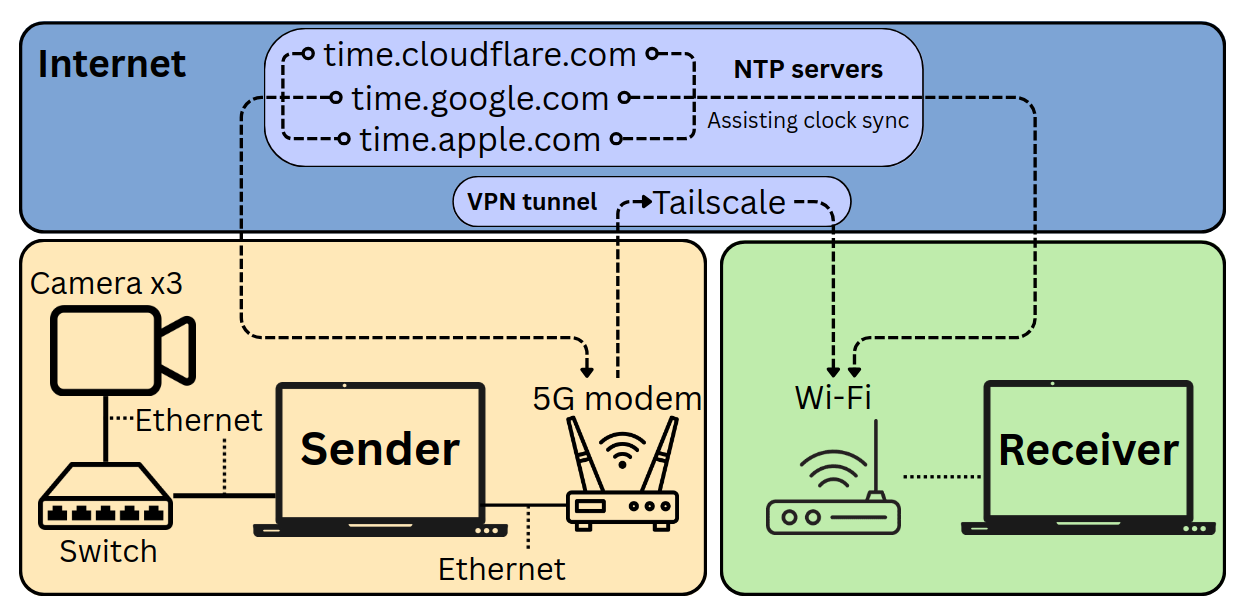
\includegraphics[width=0.9\textwidth]{Images/System/PhysicalSetup2.png}
    \caption{Physical Setup of Project}\label{fig:physicalSetup}
\end{figure}

At the application layer, the sender pulls video from each camera using RTSP over TCP, passing the video stream through a network switch into the same ethernet interface on the computer where it is transcoded or re encoded with the active configuration, packages the result into RTP, and transmits it to the receiver over UDP (or TCP for specific configurations). The receiver listens on a dedicated UDP port per camera, depay loads the RTP stream, decodes the video, and renders it to the display. Clock timestamps injected at the sender are compared against arrival timestamps on the receiver to compute end-to-end latency.

\begin{figure}[H]
    \centering
    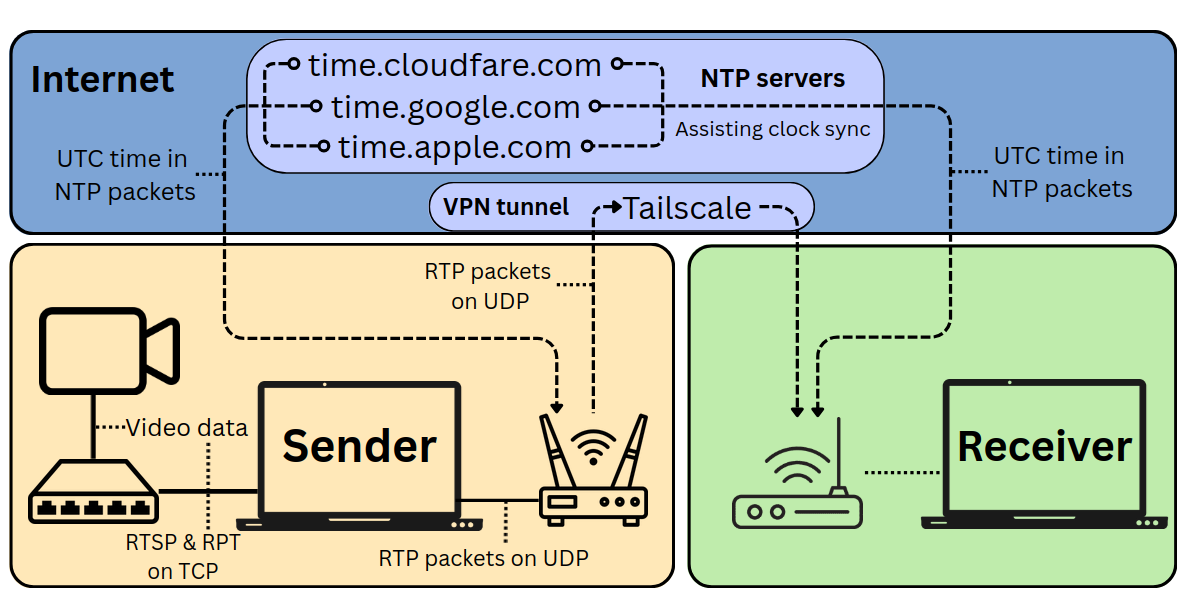
\includegraphics[width=0.9\textwidth]{Images/System/ApplicationAndTransportSetup2.png}
    \caption{Application and Transport Layer Setup of Project}\label{fig:appAndTransSetup}
\end{figure}

\subsection{Components}

The system is built from the following physical and software components.

\textbf{Cameras.} Three Hikvision DS-2CD2T47G2-L IP cameras serve as the video sources. They are managed through three tools provided by Hikvision: SADP, which is used to discover and initially configure cameras on the network. iVMS-4200, which provides a full management interface for stream settings and encoding parameters. And the Hikvision web interface, accessible directly through a browser once the camera has a known IP address. Each camera is assigned a static IP address through these tools and will retain that address until manually changed. The cameras encode video internally using either H.264 or H.265 and expose the stream over RTSP on TCP port 554. The internal encoder settings, including resolution, bitrate, frame rate, and keyframe interval, can be adjusted through the management interface, and the values used as the standard configuration for testing are listed in Chapter~\ref{sec:methodology} Table~\ref{tab:camera_stream_config}.

\textbf{Network switch.} The three cameras connect to the sender through a TP-Link TL-SG108E 8-port Gigabit Easy Smart Switch. The switch provides eight RJ45 ports with auto-negotiation at 10/100/1000 Mbps and a total switching capacity of 16 Gbps. It supports port-based QoS and VLAN configuration through a web interface. All three cameras and the sender computer share a single physical Ethernet interface on the sender side through the switch, with each camera individually addressable by its static IP address on the same subnet.

\textbf{Sender computer.} A Lenovo ThinkPad laptop running Ubuntu 24.04 LTS acts as the sender. It is equipped with an Intel Core i7 processor and 16 GB of RAM, along with a dedicated NVIDIA GPU that enables hardware accelerated video encoding. The machine connects to the camera switch over one Ethernet interface and to the 5G modem over a second Ethernet interface. The GStreamer sender pipeline runs on this machine, pulling video streams from all three cameras, processing and encoding them according to the active configuration, and forwarding the resulting RTP packets to the receiver over the internet.

\textbf{5G modem.} A Teltonika TRB500 industrial 5G gateway provides the sender with internet connectivity. The TRB500 supports 5G Sub-6 GHz connectivity with theoretical download speeds of up to 3.3 Gbps and upload speeds of up to 900 Mbps, and falls back automatically to 4G LTE and 3G when 5G coverage is unavailable. The modem connects to the sender computer over a single Gigabit Ethernet port and handles all routing between the sender and the internet. Using a 5G modem is necessary as it simulates possible equipment mounted on a moving train communicating with a fixed remote operator station over a cellular connection.

\textbf{Receiver computer.} A Dell Precision 3591 laptop running Ubuntu acts as the receiver. It is built around Intel Core i7 processor, paired with up to 16 GB of DDR5 memory. The machine connects to the internet through a standard Wi-Fi router and was stationed at a fixed NTNU lab location for the duration of all experiments, simulating a remote operator control room.

\subsection{Architecture}

\subsubsection{Network Addressing and Subnet Design}

All three cameras are connected to the sender through the TP-Link switch and share a single physical Ethernet interface on the sender computer. Each camera is assigned a static IP address within the same subnet, allowing the sender to address each one individually over that shared interface. Static addresses were chosen over DHCP because the system needs to know the exact IP address of each camera before opening an RTSP session, and a dynamic address that changes between power cycles would require additional discovery logic before every test run. Keeping the addresses fixed simplifies the startup procedure and makes the configuration reproducible across sessions.

\subsubsection{Separation of Camera Network and Internet Uplink}

The sender computer uses two separate Ethernet interfaces for two fundamentally different purposes. One interface connects inward to the camera switch and carries only RTSP and RTP traffic from the cameras. The other connects outward to the 5G modem and carries the processed RTP streams toward the receiver over the internet. This separation ensures that the camera traffic and the outgoing stream traffic never compete on the same interface which can cause data loss issues and degrade teh system, and it keeps the camera subnet entirely isolated from the public network making it more secure to others tapping into camera feed.

\subsubsection{Camera to Sender}

Between the cameras and the sender, the transport is with TCP. The sender initiates an RTSP session with each camera which negotiates the stream parameters and then delivers video data as RTP encapsulated within the same TCP connection. Channel 0 of the connection carries RTP video data and Channel 1 carries RTCP which provides control information. TCP is appropriate on this segment because the connection is a short and wired link through the switch where packet loss and reordering are negligible, and with very high bandwidth. The reliability guarantee that TCP provides simplifies session management.

The network addressing used to connect the three cameras to the sender is summarised in Table~\ref{tab:ipsetup}.

\begin{table}[H]
    \centering
    \caption{Setup for IP and Port Connection.}\label{tab:IP_and_port_Connection}
    \begin{tabular}{|c|c|c|c|c|c|c|}
    \hline
    Camera & Camera IP & Connection interface & Local IP  & Receiver IP & RTP Port\\
    \hline
    Camera 1 & 192.168.0.100 & \multirow{3}{*}{enp0s31f6} & \multirow{3}{*}{192.168.0.50} & \multirow{3}{*}{100.70.208.109} & 5000\\
    \cline{1-2}\cline{6-6}
    Camera 2 & 192.168.0.101 & & & & 5002\\
    \cline{1-2}\cline{6-6}
    Camera 3 & 192.168.0.102 & & & & 5004\\
    \hline
    \end{tabular}
\end{table}

The sequence diagram in Figure~\ref{fig:seqDiagramRTSP} illustrates the exchange that takes place between the sender and a single camera before an active video stream begins. The sender first pings the camera IP address to confirm reachability and uses NetCat to verify that RTSP port 554 is open. It then sends an RTSP DESCRIBE request, to which the camera responds with a description of the available streams. The sender follows with RTSP SETUP and PLAY requests, after which the camera begins delivering video data as RTP over the established TCP connection.

\begin{figure}[h]
    \centering
    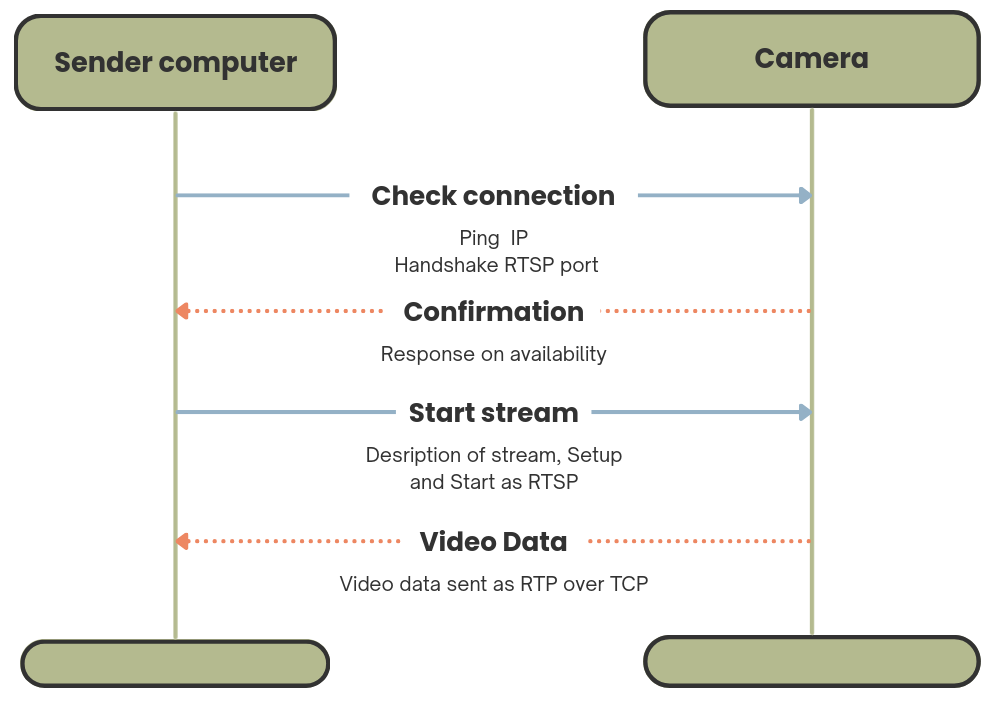
\includegraphics[width=0.9\textwidth]{Images/System/SequenceDiagramCompCam.png}
    \caption{Sequence Diagram between Sender and Camera before Active Stream}\label{fig:seqDiagramRTSP}
\end{figure}

\subsubsection{Sender to Receiver}

Between the sender and the receiver the default transport is UDP. Once the sender has received a stream from a camera and processed it according to the active configuration, it packages the result into RTP packets and transmits them to the receiver over the internet via Tailscale. UDP was chosen for this segment because it introduces no connection setup overhead and no retransmission delay which would add directly to end-to-end latency and was prioritised over the possibility of lost packets.

\subsubsection{Tailscale as a Network Overlay}

The sender connects to the internet through a 5G modem using a dynamically assigned cellular IP address, while the receiver connects through the university Wi-Fi network. Both of these addresses can change between sessions, and the university network blocks direct peer-to-peer connections between devices making it impossible to address the receiver directly from the sender without an intermediary. Tailscale solves all of these problems at once. It assigns each machine a stable virtual IP address in the 100.x.x.x range that does not change regardless of which physical network the machine is connected to. Tailscale establishes a direct encrypted WireGuard tunnel between the two endpoints so that traffic does not pass through a central server, and it operates transparently over the university network without requiring any firewall exceptions or port forwarding. The result is that the sender can always reach the receiver at a fixed address as if both machines were on the same local network, regardless of where either machine is physically located. The encrypted tunnel is an additional benefit of WireGuard but was not the primary motivation for using Tailscale in this setup.

Tailscale and WireGuard do introduce some additional latency compared to a direct connection, as every packet must pass through the encrypted tunnel and be processed by the WireGuard protocol on both ends before being delivered. The overhead is generally small, but it is a consistent addition to every packet and cannot be removed from the measurement results. Running all tests through Tailscale means this overhead is present equally across all configurations, so the results remain comparable to each other, but the absolute latency values will be slightly higher than what a direct connection would produce. The virtual IP layer also adds a small amount of packet size overhead to every transmitted frame, which is necessary to account for when applying the bandwidth constraints in the limited bandwidth test conditions.

\subsection{Pipeline Design}

\subsubsection{GStreamer}

GStreamer is an open source multimedia framework built around a modular pipeline architecture where every processing step is provided by a plugin element, and individual elements can be connected freely to form a complete processing pipeline suited to the application at hand. It runs natively on Linux and has broad support for the codecs, transport protocols, and hardware acceleration interfaces relevant to this project.

An advantage of GStreamer for this project is the access it provides to the data flowing through the pipeline. Every buffer that passes through a GStreamer pipeline carries a timestamp, and probes can be attached to any pad at any point in the element without modifying the pipeline structure itself. This makes it possible to record the precise time a packet leaves the sender and the precise time the corresponding decoded frame arrives at the receiver, which is the measurement approach used throughout this project. Running separate pipeline instances per camera rather than a single merged pipeline keeps failure isolated, so a problem on one stream does not interrupt the others, and scaling to three cameras requires only duplicating a pipeline instance rather than restructuring any shared logic.

Using GStreamer also makes the system easy to reconfigure between test runs. Swapping a codec, transport protocol and SRTP encrypting requires replacing a few elements in the pipeline while everything upstream and downstream remains unchanged. This modularity was important given the iterative development approach described in Section Development Methodology where each sprint introduced a new configuration variant that needed to be testable with minimal disruption to the rest of the system.

GStreamer does include a significant learning curve for development. The interactions between element properties, capabilities, and pipeline state transitions require careful understanding and a lot of testing before a pipeline behaves as expected. Debugging a pipeline that fails to link or silently drops buffers has consumed considerable time, and documentation quality varies across plugin elements. Several development sprints were spent resolving compatibility issues. Yet, for a project where precise instrumentation, flexible reconfiguration, and multi-stream scalability are main requirements GStreamer provides capabilities that simpler tools do not.

\subsubsection{Sender Pipeline}

The sender pipeline for each camera is shown in Figure~\ref{fig:senderPipeline} and follows this element chain.

\begin{figure}[H]
    \centering
    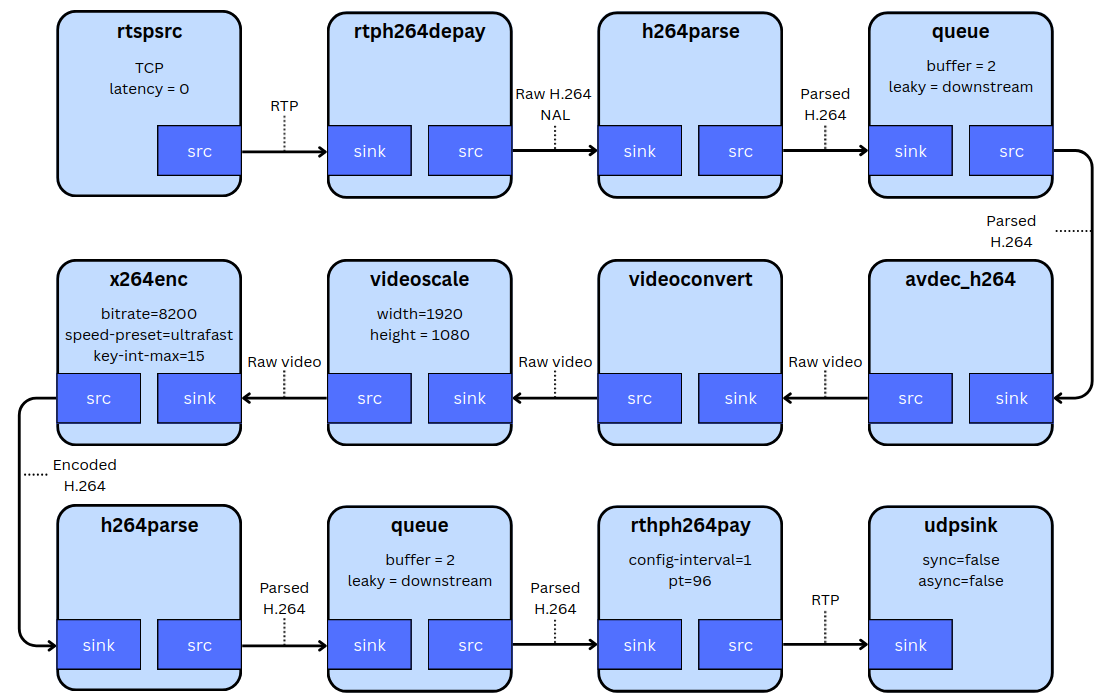
\includegraphics[width=0.9\textwidth]{Images/System/SenderPipeline.png}
    \caption{Sender Pipeline for Each Camera Stream}\label{fig:senderPipeline}
\end{figure}

\textbf{rtspsrc} opens an RTSP session with the camera over TCP and pulls the incoming RTP stream. The \texttt{latency=0} is disabling the internal jitter buffer, as the wired local connection introduces negligible timing variation and buffering would only add fixed delay.

\textbf{rtph264depay} strips the RTP packaging and recovers the raw H.264 NAL units.

\textbf{h264parse} structures the NAL unit stream into a access units with verified parameter sets, ensuring the downstream decoder receives properly delimited frame boundaries.

\textbf{queue} decouples upstream and downstream elements into separate threads. This allows the previous elements to hand off the video stream to this queue and start working on the next. Creating a waiting place before avdec is ready to continue. The buffer is limited to 2 frames with \texttt{leaky=downstream}, meaning the oldest frame is dropped when the buffer is full rather than blocking the pipeline, which keeps latency bounded.

\textbf{avdec\_h264} decodes the compressed H.264 bitstream into raw YUV frames. This is necessary because the re-encoding stage downstream requires uncompressed input.

\textbf{videoconvert} and \textbf{videoscale} prepare the raw frames for encoding. Videoconvert resolves any pixel format incompatibility between the decoder output and the encoder input automatically, while videoscale resizes the frames to the target resolution enforced by the caps filter at 1920$\times$1080.

\textbf{x264enc} compresses the raw frames into a new H.264 bitstream. \texttt{tune=zerolatency} disables internal buffering and frame reordering, \texttt{speed-preset=ultrafast} minimises encoding time by allowing suboptimal quality, and \texttt{key-int-max=15} sets the keyframe interval so a receiver can recover quickly after packet loss.

\textbf{h264parse} is applied again after encoding to structure the freshly encoded bitstream before it reaches the payloader.

\textbf{queue} provides a second decoupling point between encoder and payloader, again with a 2 frame buffer and \texttt{leaky=downstream}.

\textbf{rtph264pay} packages the H.264 bitstream into RTP packets. \texttt{config-interval=1} injects SPS and PPS parameter sets into every keyframe so a receiver joining mid-stream can synchronise immediately for reliability, and \texttt{pt=96} sets the dynamic payload type for H.264.

\textbf{udpsink} transmits the RTP packets to the receiver Tailscale address on the port assigned to that camera. \texttt{sync=false} and \texttt{async=false} ensure packets are sent immediately rather than being held to match a clock reference.

\subsubsection{Receiver Pipeline}

The receiver pipeline for each camera stream is shown in Figure~\ref{fig:receiverPipeline} and follows this element chain.

\begin{figure}[h]
    \centering
    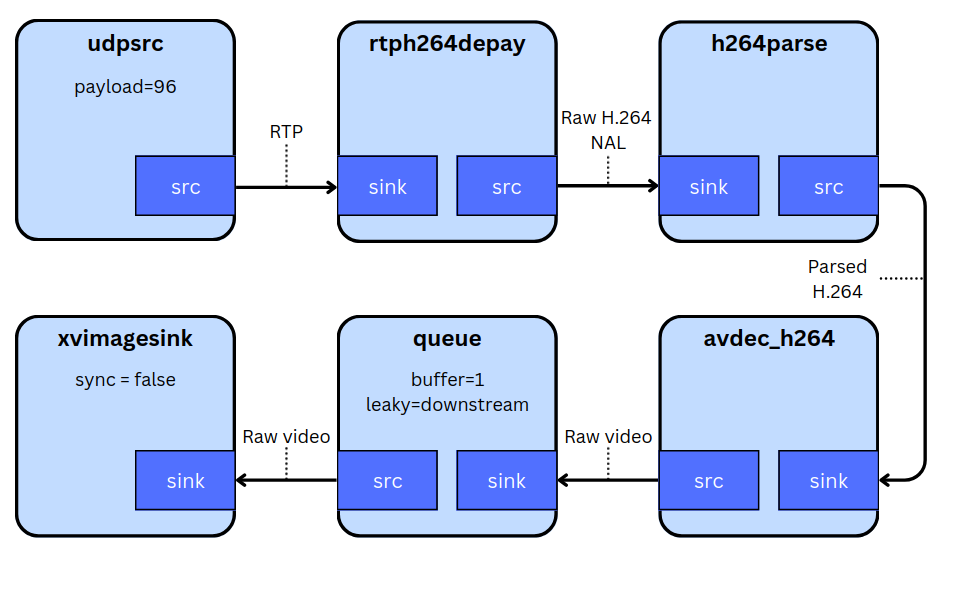
\includegraphics[width=0.9\textwidth]{Images/System/ReceiverPipeline.png}
    \caption{Receiver Pipeline for Each Camera Stream}\label{fig:receiverPipeline}
\end{figure}

\textbf{udpsrc} listens on the UDP port assigned to the camera stream. The caps property explicitly declares the expected payload format, including media type, encoding name, and payload type 96, so GStreamer can negotiate the correct downstream elements without misinterpretation.

\textbf{rtph264depay,}\textbf{h264parse,} \textbf{avdec\_h264} and \textbf{queue} provides the same value and result as in the sender. Choices of buffer size is from the iterative development phase when testing of different values resulted in 2 for sender and 1 receiver at best result.

\textbf{xvimagesink} renders each decoded frame to the display as soon as it arrives. \texttt{sync=false} disables presentation time gating, so frames are shown immediately upon decoding rather than being held to match any clock reference.

\subsection{Measurement Design}\label{sec:measurementdesign}
This section describes the implementations done to get good measurements of the system. Six distinct measurements are collected during a run of the video system, this to get a proper understanding of the trade-offs and benefits of all components tested. An important aspect of all the measurement design was to try to avoid as much noise and disturbance to the main video stream. This is done by separating measurements where possible, but also avoid writing to disk during the run. Instead everything is logged locally before after stop to write it to disk, reducing contribution of workload on the computers.

\subsubsection{Probe Placement}

Latency within the sender and receiver pipelines is measured using GStreamer probes. A probe is a callback attached to a specific pad in the pipeline that fires for every buffer passing through that point, without modifying or interrupting the data flow. This makes probes the appropriate tool for timestamping data in motion through a live pipeline. Important to note is that a probe fires every single something passes. So its very important to choose appropriate placement. Comparing Raw H.264 NAL units to RTP packets will result in a invalid measurement, this is the reason it is not possible to measure every single element in the stream. The probe placement for both pipelines is illustrated in Figure~\ref{fig:senderProbes} and Figure~\ref{fig:receiverProbes}.

On the sender, one probe is placed on the sink pad of \texttt{rtph264depay}, capturing a monotonic timestamp at the moment the first RTP packet of each incoming frame arrives from the camera. A second probe is placed on the sink pad of \texttt{udpsink}, capturing a timestamp and the RTP sequence number at the moment the corresponding outgoing packet is handed to the network. The difference between these two timestamps gives the sender pipeline latency for that frame.

\begin{figure}[H]
    \centering
    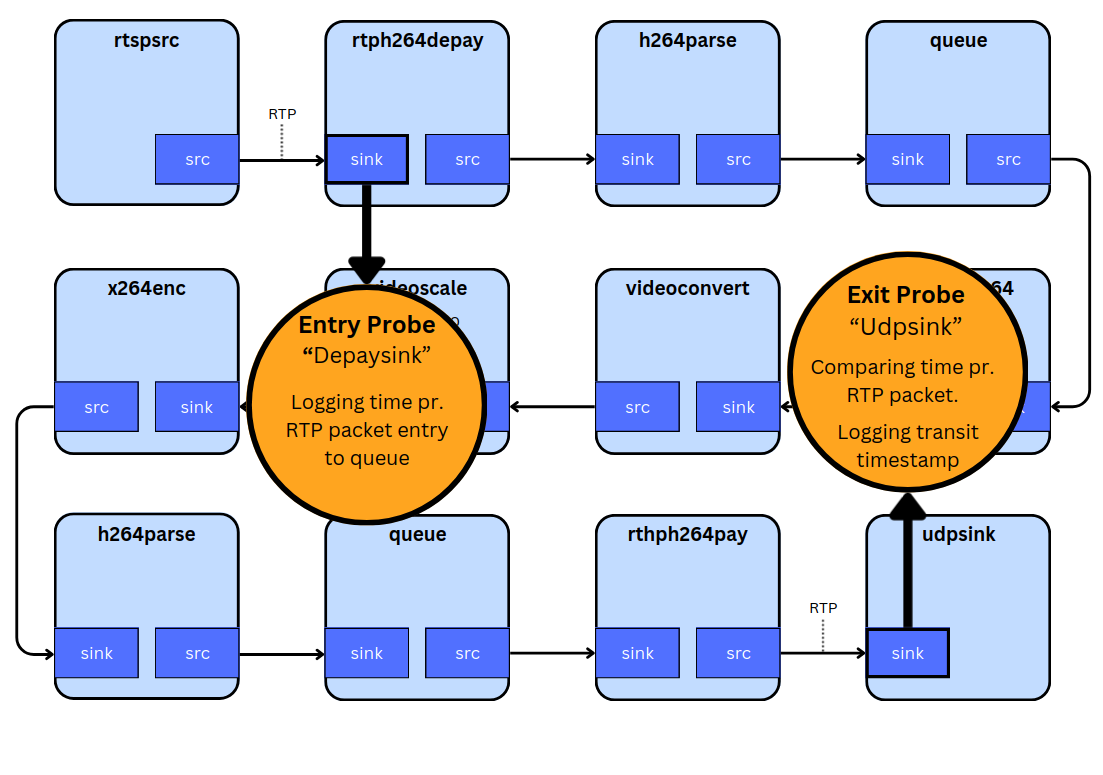
\includegraphics[width=0.9\textwidth]{Images/System/SenderProbes.png}
    \caption{Probe Placement in Sender Pipelines}\label{fig:senderProbes}
\end{figure}

On the receiver, one probe is placed on the source pad of \texttt{udpsrc}, capturing a monotonic timestamp at the moment the first RTP packet of each incoming frame arrives from the network. It also captures a transit timestamp for every RTP packet arriving. A second probe is placed on the sink pad of \texttt{xvimagesink}, capturing a timestamp at the moment the corresponding decoded frame reaches the display. The difference between these two timestamps gives the receiver pipeline latency for that frame, covering depay, parsing, decoding, and queuing on the receiver machine.

\begin{figure}[H]
    \centering
    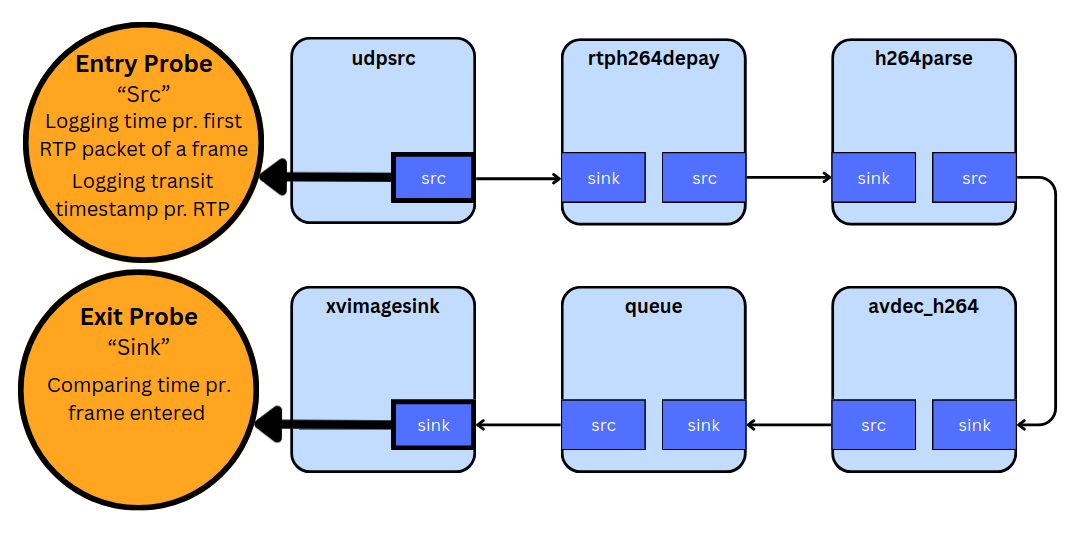
\includegraphics[width=0.9\textwidth]{Images/System/ReceiverProbes.png}
    \caption{Probe Placement in Receiver Pipelines}\label{fig:receiverProbes}
\end{figure}

The RTP marker bit is used to identify frame boundaries. In H.264 over RTP, the marker bit is set on the last packet of each frame. The sender probe timestamps the first packet of a frame on the way in and the last packet of the same frame on the way out, ensuring that the pipeline latency logged per frame reflects the full time that frame spent inside the sender processing chain.


\subsubsection{Latency measurment}
For latency measurements, three separated measurements are completed to try to pinpoint where possible issues arise. The system has sender pipeline latency, receiver pipeline latency and transit latency. As mentioned in Probe Placement, both sender and receiver pipeline measurements uses Gstreamer internal pipeline measurements tools, complete avoiding any delay of clock ticks and therefore keeping a very healthy result. Each time video data is passed through the starting probe, it logs the time in a queue list. Then at the last probe it confirms that the queue matches correct. If there are to many timestamps in the queue, that means a \texttt{leaky=downstream} has gotten rid of an image, and a log of dropped image is recorded. It then compare time now and the time in the queue, calculating the full pipeline measurement.

Transit latency across the network is measured by timestamping when an RTP packet leave the sender computer, and timestamping when it enters the receiver. These points of entry and exit are also the same points the sender and receiver pipeline measure internal latency to make sure of no missed end-to-end latency. The logged transit times are compared on RTP sequence number to differentiate the packets before comparing and computing latency.

\begin{equation}
  L_{\text{transit}}  = T_{\text{receiver}} - T_{\text{sender}}
\end{equation}

\subsubsection{Clock synchronisation design}
Originally two GPS clock synchronisers were in use. They were implemented to get a more accurate transit latency by making sure that both computers are following the same clock and avoid clock shifts. In the beginning a method where the GPS signal, including time was parsed, integrated in the RTP packet and then sent was used. With further testing, the parsing and implementations of the timestamp was an additional added latency and workload for the computer, not to mention responsible for higher throughput. Another system was tested where the pipeline works in the same way as now, by using the computer timestamp to log. The idea was for the GPS clock to overwrite the internal computer clock, which worked. But unfortunately the GPS clocks had a low Hz so the overwriting only occurred a couple times per second allowing the clock to drift anyway, and introduced a unstable margin of error as it would jump from 20~ms off to 0~ms off before slowly drifting again. After that, the usage of internet NTP servers to help correct the internal clock when drifting was used. It resulted in a stable, and mild offset that could be used for measurement.

\subsubsection{Packet loss}
Packet loss uses the same logging as the transit latency. When comparing and computing the transit latency. The code counts all packets sent and received and find the difference before computing the percentage by doing difference divided by total sent. The code that computes also avoids the first 10 seconds of sender logs. This to avoid any startup issues. The receiver packets then without any sender logs for the beginning is also ignored ensuring a healthy measurement.

\begin{equation}
  \text{Packet loss}_{[\%]} = \frac{Packets_{\text{sent}} - Packets_{\text{received}}}{Packets_{\text{sent}}}
\end{equation}

\subsubsection{Visual Quality Measurement}

Visual quality is assessed on the receiver using the BRISQUE score. BRISQUE is a no-reference image quality metric that assigns each frame a score between 0 and 100, where a lower score indicates a frame that more closely resembles a natural, undistorted image. It operates entirely on the decoded frame without needing access to an original reference image, making it suitable for a live streaming context where no ground truth is available.

A \texttt{tee} element on the receiver splits the decoded video stream after \texttt{avdec\_h264} into two branches. One branch leads to \texttt{xvimagesink} for display. The other passes through \texttt{videoconvert} to produce a raw BGR frame and into an \texttt{appsink}, which makes the frame available to Python code for BRISQUE scoring as you can see in Figure~\ref{fig:BRISQUEProbe}. The \texttt{appsink} is configured with \texttt{drop=true} and \texttt{max-buffers=1} so that it never blocks the display branch, dropping frames it cannot process in time rather than introducing pressure back into the pipeline. To keep CPU load manageable, only every fifth frame is scored.

\begin{figure}[H]
    \centering
    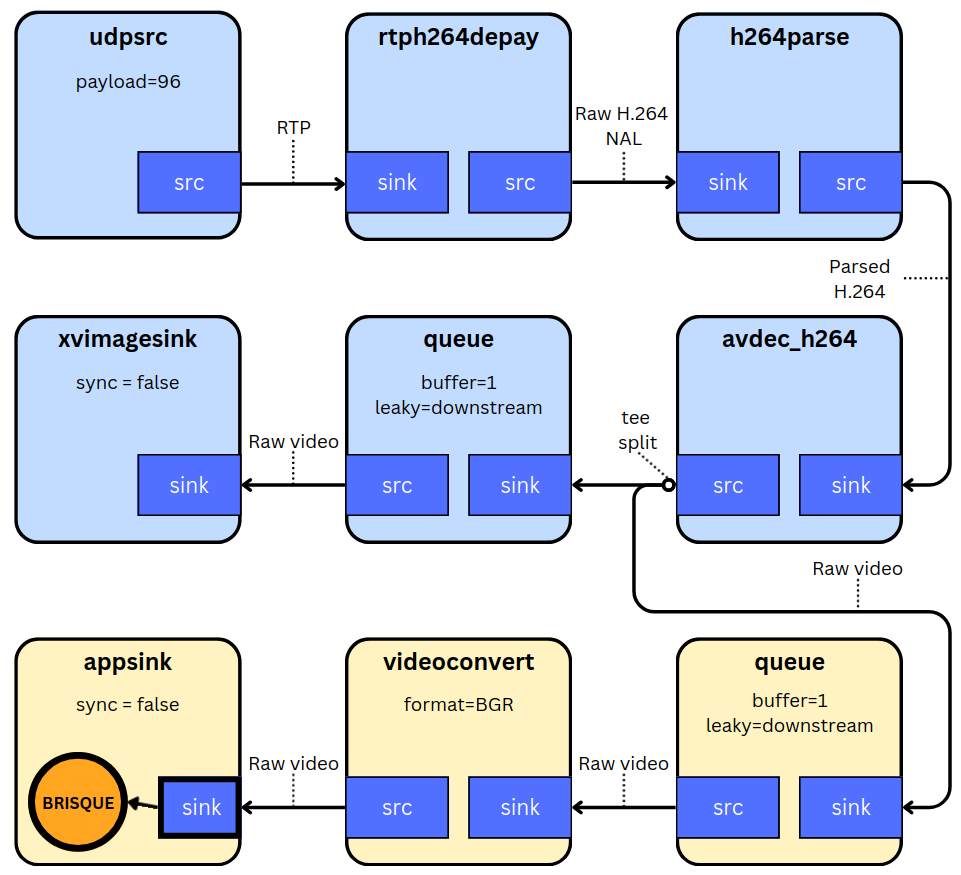
\includegraphics[width=0.9\textwidth]{Images/System/BRISQUEProbe.png}
    \caption{BRISQUE extended pipeline for receiver}\label{fig:BRISQUEProbe}
\end{figure}

\subsubsection{CPU Usage Measurement}

CPU usage is logged on the sender using \texttt{sar}, a standard Linux system activity reporter that records processor usages at a fixed interval. It is configured to sample all CPU cores once per second for the full duration of each test run and writes the output directly to a log file. Running \texttt{sar} as a separate process alongside the GStreamer pipeline ensures that the measurement tooling does not share threads with the pipeline itself, meaning the act of logging CPU usage does not influence the CPU load being measured.

CPU usage is recorded on the sender only, as encoding is the computationally demanding operation in this system. The receiver workload is comparatively low and consistent across configurations, making it less relevant for distinguishing between test cases.

\subsubsection{Throughput Measurement}

Outbound throughput on the sender is measured by reading \texttt{/proc/net/dev} once per second from a dedicated background thread. This file is maintained by the Linux kernel and contains cumulative byte counters per network interface. By computing the difference in transmitted bytes between consecutive readings and converting to megabits per second, the thread produces a continuous record of how much data the sender is pushing toward the receiver over the Tailscale interface throughout each test run.

Measuring throughput on the Tailscale interface specifically, rather than on the physical network interface, captures only the traffic directed at the receiver and excludes any background traffic on the same physical link. This keeps the throughput values directly comparable across test configurations and directly tied to the video streams under evaluation.

\subsubsection{Data Recording}

All probe measurements are written to CSV log files by a dedicated background writer thread on each machine. Using a separate thread ensures that file I/O does not block the probe callbacks, which run on GStreamer pipeline threads where any delay would affect the very latency being measured. The sender produces two log files per run, one for sender pipeline latency per frame, one for transit timestamps, CPU usage and throughput. The receiver produces three log files per run, one for receiver pipeline latency, one for transit timestamps, and one for BRISQUE quality scores.